\ofsubsection{Tomb of Raithwall}
%
\ofquote{"Though he is called the Dynast King, upon establishing the alliance, he  showed compassion for his people, and disdain for war. A philosophy passed on to his successors. One that would bring peace and prosperity for hundreds of years to follow."}{Ashe}\\\\
%
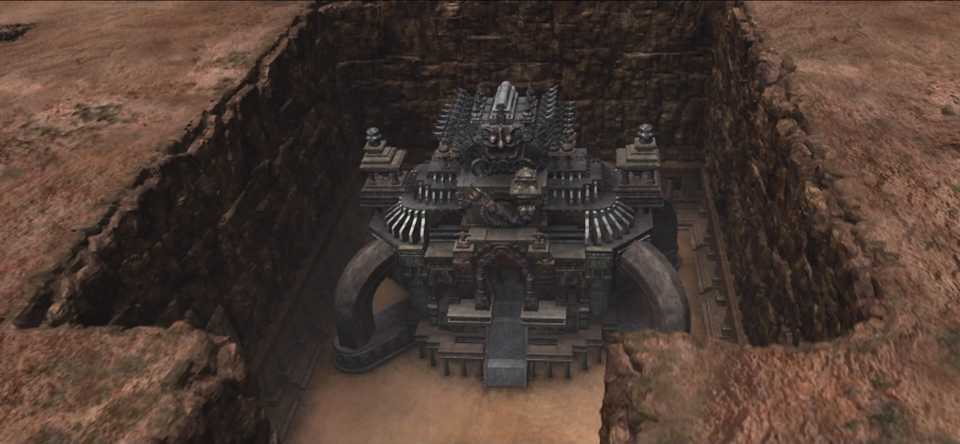
\includegraphics[width=\columnwidth]{./art/tombofraithwall/tomb1.jpg}
%
\ofpar
%
\accf{Tomb of Raithwall} is a pre-prepared adventure that is self-contained and can be played either standalone or integrated into a larger campaign.
In this adventure, the party explores an ancient tomb in search of a powerful artifact of legends.
Tomb of Raithwall is designed for a Level 3 party, but depending on factors such as party size and experience, you may need to adjust some of the enemies and rewards.
In case the players create new Level 3 characters, they can use the standard rules for choosing starting equipment and everyone receives an additional 1500G in cash.
Also, the story of every character should explain why he or she joined this dangerous treasure hunt.
Note that detailed maps of the tomb are given at the end of this document.
%
\ofpar
%
\ofquote{"There's no guarantee we'll make it out alive. Vicious beasts. Fiendish traps. Something like that?"\\}{Balthier}\\\\
%
After a march through the vast Nam-Yensa Sandsea, the party arrives in front of a tall cliff and they spot a narrow gap leading inside.
Next to this entrance, they meet the traveling merchant \accf{Dyce} who has enacted a camp.
Dyce is a well built, tall man, bald with beard and wears a dark outfit, he also has a Chocobo at his side that he travels on.
He informs the party that the path through the cliffs leads to the Tomb of Raithwall and tells them about its history:
The tomb is the resting place of \accf{King Raithwall}, also called the Dynast King.
Legends say that in ancient times, Raithwall was a generous king who united many warring kingdoms under his banner, bringing peace and prosperity to the land.
It is believed that the key to his power was a magical artifact, named the \accf{Dawn Shard}.
According to the legend, with his last breath, King Raithwall sealed the tomb with himself and the Dawn Shard inside to prevent its power from falling into the wrong hands.
Many adventurers have tried to claim the Dawn Shard, but they only found their doom in the many dangers and traps of the tomb.
Through further inquiry, the party can find out that Dyce is not here by coincidence, in fact he is hoping to profit of the many adventurers passing through this spot.
As such, he also offers to sell his goods to the party, at a 50\% higher price compared to regular stores (he calls this the "risk premium").
Dyce also assures the party that he will remain in this spot for some time, in case they need to make more purchases in the future.
He has the following Items and Accessories in his inventory: Potion, Ether, Hi-Potion, Turbo Ether, Phoenix Down, Light Curtain, Lunar Curtain, Rune Bracers, Mythril Shield, Silver Glasses, White Cape, Star Pendant.
%
\vfill
%
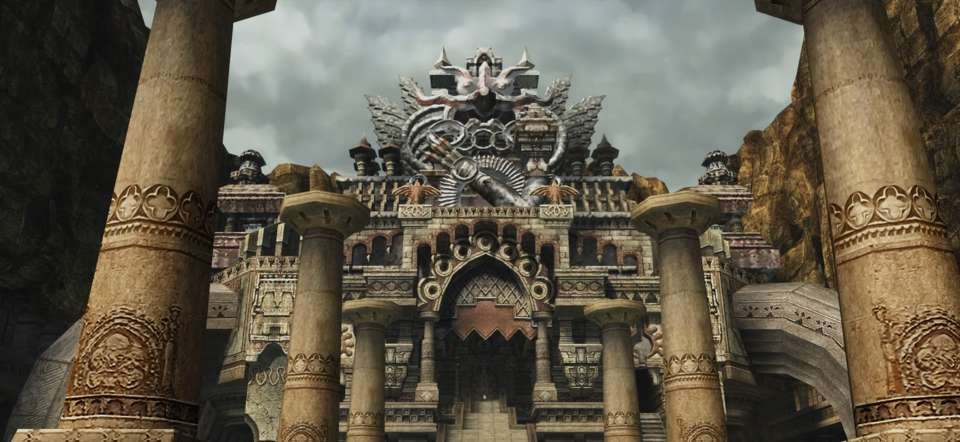
\includegraphics[width=\columnwidth]{./art/tombofraithwall/tomb2.jpg}
%
\vfill
%
After the party steps through the narrow gap in the cliffs, they find themselves in the so-called \accf{Death Valley} with the massive tomb right in front of them.
A set of tall stone pillars on both sides mark the way to a long flight of stairs leading into the Tomb of Raithwall.
As the party makes it half way through the valley, they are suddenly disturbed by a deafeningly loud screeching and a huge bird-like creature descends upon them.
\accf{Garuda} as one of the many guardians of the tomb, protects its entrance in the ensuing fight.
Only after defeating the beast, the party can make their way into the tomb through the central flight of stairs.
%
\vfill
%
\ofmonster{Garuda}{3}{
\includegraphics[width=0.3\columnwidth]{./art/monsters/garuda.png}}
{
	HP: & \hfill 50 & MP: & \hfill 120\\
	STR: & \hfill 3 & DEF: & \hfill 2 \\
	MAG: & \hfill 4 & RES: & \hfill 3 \\
	AGI: & \hfill 2 & Size: & \hfill L\\
}
{\accf{Beak}: 2d DMG \hfill \accf{Drops:} 800G, Phoenix Down \\ \accf{Resilient:}\wind \hfill \accf{Immune:}\poison\sleep\immobile \hfill \accf{Weak:\lightning}}
{
	\mspell{Aero}{8}{0r}{Single}{4u}{You deal 2d wind damage to the target.}{\wind}
	\mspell{Aerial Blast}{10}{1r}{10u (line)}{Self}{All enemies in the target area suffer 4d wind damage.}{\wind}
	\mtech{Fly}{4}{0r}{Single}{Self}{You ascend up to a height of 3u. While in the air, you can move as usual. After 3 rounds, descend next to an enemy within 8u and make an Attack on him.}{}
	\mpassive{Wing Slap}{Whenever you make an Attack against an enemy within range, you can also make second Attack against another enemy within 2u.}
}
%
\clearpage
%
\ofquote{"Fight or run, we better decide fast!"\\}{Vaan}\\\\
%
After entering the tomb, the party find itself inside a large hall, the \accf{Hall of the Destroyer}.
Its entrance is built on an elevated platform and by using one of two parallel stairways the party reaches the central corridor that leads further into the tomb.
On their way, they notice that the tomb is lit by many fire sources such as torches and fire pits that seem to burn perpetually and in an unnatural manner, presumably through magical means.
Moreover, they pass a heavily decorated piece of wall, with what looks like the statue of a monster sunk into it, looking into the corridor.
Suddenly, as they step into the corridor, the ground begins to shake and a loud noise emerges from behind them.
As they turn around, the party is confronted with the massive wall that has come alive to block the path to the entrance.
%
\vfill
%
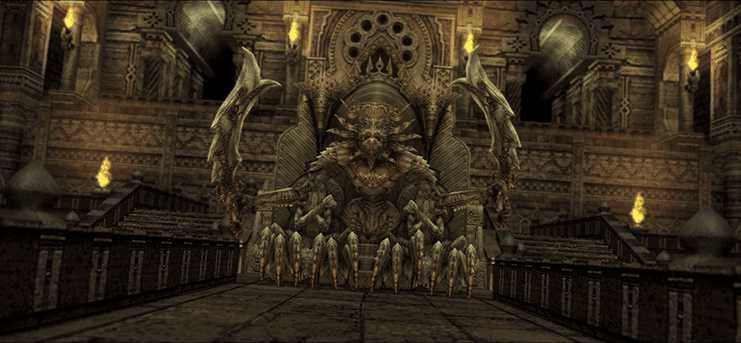
\includegraphics[width=\columnwidth]{./art/tombofraithwall/demonwall2.jpg}
%
\ofpar
%
\accf{Demon Wall} is another guardian of the tomb and in the ensuing fight, he keeps moving forward on every turn, pushing the party towards the opposite side of the corridor.
He receives no surprise round, but takes the first turn.
The party cannot walk past Demon Wall, because it blocks the entire passage, so they either have to defeat it or flee through the door on the other side.
When a player reaches the heavy double door, he has to use his action and pass a DC~8 check to open it.
Upon failure, he is only able to move the door a little bit, but the next one to try the same receives Advantage on the check.
When Demon Wall reaches the door, it closes in and crushes everyone in the way. 
After some time, Demon Wall retreats to its original position, but whenever the party steps through the corridor again it emerges and Attacks in the exact same manner.
However, it does not regenerate any HP, so the party can try to wear it down over multiple attempts.
You can describe that parts of it are crumbling and breaking to visualize the damage that Demon Wall takes.
The party does not immediately have to defeat Demon Wall, but they have to do so eventually as it blocks the only entrance out of the tomb.
A major advantage of defeating it early is that it allows the party to step outside either to rest or to buy more Items from Dyce.
%
\newpage
%
\ofmonster{Demon Wall}{4}{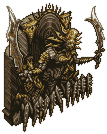
\includegraphics[width=0.2\columnwidth]{./art/monsters/demonwall.png}}
{
	HP: & \hfill 100 & MP: & \hfill 150\\
	STR: & \hfill 4 & DEF: & \hfill 3 \\
	MAG: & \hfill 3 & RES: & \hfill 4 \\
	AGI: & \hfill 2 & Size: & \hfill L\\
}
{\accf{Swords}: 2d DMG, \hfill \accf{Drops:} 1000G, Hi-Potion \\ \accf{Resilient:}\earth \hfill \accf{Immune:}\poison\sleep\blind \hfill \accf{Weak:\water}}
{
	\mspell{Poison}{6}{0r}{Single}{5u}{The target makes a DC~8 check and suffers Poison for 3 rounds upon failure.}{}
	\mspell{Blind}{6}{0r}{Single}{5u}{The target makes a DC~8 check and suffers Blind for 3 rounds upon failure.}{}
	\mspell{Silence}{6}{0r}{Single}{5u}{The target makes a DC~8 check and suffers Silence for 3 rounds upon failure.}{}
	\mspell{Slow}{8}{0r}{Single}{5u}{The target suffers Slow for 3 rounds.}{}
	\mpassive{Quickcast}{Whenever you make an Attack, you can cast a spell immediately afterwards.}
	\mpassive{Push}{Whenever you walk forward, push away all enemies in your path. You can use this ability to crush enemies between yourself and a wall or door, immediately causing them KO.}
}
%
\vfill
%
\ofquote{"But you must consider the prize. The Dawn Shard lies within. And Raithwall's treasure."\\}{Ashe}\\\\
%
After passing through the door, the party finds themselves in a chamber called the \accf{Royal Passage}.
On the other side of the room, they notice a decorated double door, which the party is unable to open at present.
The door also has two circle shape cavities on it, one on each wing. 
To the left and right side of the room, there are two smaller stairways leading downwards.
Additionally, the party notices a mural that has been engraved into the floor of the room, it shows a man holding up an object, a bird to his left and a wall to his right.
The image is supposed to depict the creation of Garuda and Demon Wall through the use of the Dawn Shard.
Furthermore, next to the door they came in from, the party notices a man lying on the ground.
He seems to have succumbed to his heavy wounds and upon closer inspection, they can deduce that he fell victim to Demon Wall.
From the way he is dressed, he gives the impression of being a bandit or grave robber, the party can loot the following from him:
an Advanced Level weapon (pick something one of the players can use), 500G and 2 Potions.
To progress further, the party has to explore the Northfall and the Southfall passages through the stairs in this room. 
However, before they set off, every player receives a \accf{Level Up}!
%
%
\clearpage
%
\ofquote{"In vainglory they arose, shouting challenges at the gods. But prevail they did not. Their doom it was to walk the mist until time's end."\\}{Fran, reciting a legend}\\\\
%
If the party takes the stairs on the right hand side of the Royal Chamber, they find themselves inside a large corridor of the \accf{Northfall Passage}.
Most of the floor in this room has a checkerboard pattern with black and white tiles, the right hand side wall is black while the left hand is white colored.
Furthermore, the left wall contains a row of cone shaped cavities at a height of roughly 1u.
In case the party investigates the room in more detail, they notice that the black tiles are slightly elevated and the cavities on the left wall have holes in their center.
The room is a trap, as soon as the party steps on any of the black tiles, the cones on the left wall start spraying fire.
If the trap is sprung, every party member makes a DC~9 check to decide whether they can duck quickly enough and every one who fails, suffers 3d fire damage.
The trap can be avoided by only stepping on the white tiles or by crawling on the ground.
%
\vfill
%
After the corridor, the party enters a larger chamber that is empty, except for six stone sarcophaguses that are spread across the room.
As they enter, the players notice the words \accf{"GUARDIANS OF THE ARMOR"} engraved into the floor.
Once the players move towards the other side of the room, suddenly the sarcophaguses break open and a set of mummies emerge from them to attack the party.
The number of mummies should be equal to the party size and in the ensuing fight they gain a surprise round.
However, if the players tried to investigate a sarcophagus beforehand, they gain the upper hand against the ambush and thus the surprise round.
After defeating the enemies, the party can investigate the now open sarcophaguses to find the following items: a Power Armlet, 2 Hi-Potions and a Turbo Ether.
The room has two exits, one to the right hand side and another one opposite to the entry.
%
\vfill
%
\ofmonster{Mummy}{4}{
\includegraphics[width=0.18\columnwidth]{./art/monsters/mummy.png}}
{
	HP: & \hfill 38 & MP: & \hfill 0\\
	STR: & \hfill 2 & DEF: & \hfill 3 \\
	MAG: & \hfill 1 & RES: & \hfill 1 \\
	AGI: & \hfill 2 & Size: & \hfill M\\
}
{
	\accf{Bite}: 2d DMG \hfill \accf{Drops:} 300G, Potion  \\
	\accf{Immune}:\poison\sleep \hfill \accf{Weak}:\fire 
}
{
	\mspell{Blizzard}{4}{0r}{Single}{3u}{The target suffers 2d ice damage.}{}	
	\mpassive{Zombietouch}{Whenever you successfully Attack a target he makes a DC 8 check and suffers Zombie for 1~hour upon failure.}
	\mpassive{Undead}{You permamently suffer the Zombie status.}
}
%
\newpage
%
By passing through the door on the right hand side, the party steps into a long corridor and upon entering they notice two chests on the left hand side.
One is made out of wood and its lock can easily be broken by force, it contains a Bomb Fragment and an Ether.
The other chest is made out of metal and cannot be opened by force, instead characters can attempt to pick its lock by passing a DC~8 check.
After unlocking it, the party finds a MP Plus Materia and a Phoenix Down inside the chest.
The corridor seems to lead to a dead end, but the wall at its end is decorated with a very striking image: it depicts King Raithwall using powerful fire magic against a monster.
Upon closer inspection, the party notices that the fire depicted in the image emits a faint red glow, presumably of magical nature.
If they deal any fire damage to the wall, a magical mechanism is activated that opens up a small gap in the wall, revealing a secret room.
In the middle of this small room stands a pedestal on which the party finds a Fire Cufflink Accessory as well as a Dragon Materia.
%
\vfill
%
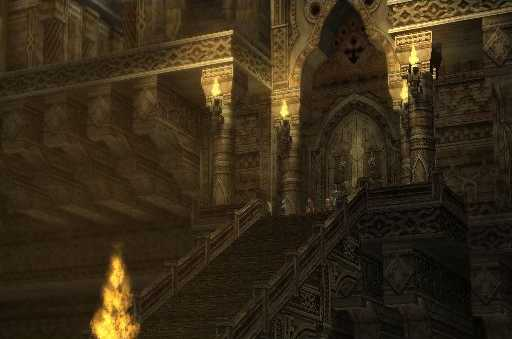
\includegraphics[width=\columnwidth]{./art/tombofraithwall/tomb5.jpg}
%
\vfill
%
After walking through the other door past the sarcophaguses, the party enters a large room with a statue at its center, which is roughly 2u in height.
The statue depicts King Raithwall clothed in heavy armor and his arm is stretched out as if he was holding a weapon, however his hand is empty.
In front of the statue is a pedestal with a set of heavy armor on it which looks very similar to the armor that the statue is wearing.
The walls in this room are engraved with images of King Raitwall fighting various monsters with a decorated longsword.
When the party recovers \accf{Raithwall's Sword} from the Southfall Passage and puts it in the hand of the statue in this room, they hear a soft noise, as if a mechanism has been activated.
After solving the puzzle in this room and making their way back to the Royal Chamber, they notice that one of the two engravings on the sealed door has now started glowing.
The armor on the pedestal is \accf{Raithwall's Armor}, which the party needs for the Southfall Passage.
However, after solving the complete puzzle and opening the sealed door, they may claim the armor, in this case it is treated as an Advanced level heavy armor that increases its wearer's maximum MP by 10.
%
\clearpage
%
\ofquote{"Call me old-fashioned, but i was hoping for a treasure whose worth we COULD measure."\\}{Balthier}\\\\
%
If the party takes the stairs on the left hand side of the Royal Chamber, they find themselves in the \accf{Southfall Passage} which consists of two rooms.
The first one is a very big hall with two doors on the opposite side of its entrance.
As they enter, the players notice the words \accf{"GUARDIANS OF THE SWORD"} engraved into the floor.
Towards the center of the hall stand three pairs of large Gargoyle statues on opposite sides of the room facing each other.
Furthermore, faint red lines are drawn on the ground that connect each pair and in case a player crosses a red line, the two Gargoyle statues connected to it come alive and attack the party.
However, there is also some space behind each statue, so the players can avoid the traps by walking along the walls instead of through the center of the room.
If the party manages to reach the other end of the hall without triggering any statue, they suddenly hear a faint noise as the red lines on the ground disappear.
Moreover, a small compartment opens up at the pedestal of the statues in total containing the following treasures: 1000G, 3 Light Curtains and 3 Lunar Curtains.
%
\ofpar
%
\ofmonster{Gargoyle}{4}{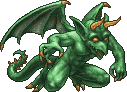
\includegraphics[width=0.27\columnwidth]{./art/monsters/gargoyle.png}}
{
	HP: & \hfill 38 & MP: & \hfill 30\\
	STR: & \hfill 3 & DEF: & \hfill 2 \\
	MAG: & \hfill 0 & RES: & \hfill 0 \\
	AGI: & \hfill 2 & Size: & \hfill M\\
}
{	
	\accf{Claw}: 2d DMG \hfill \accf{Drops:} 300G\\
	\accf{Resilient}:\earth \hfill \accf{Weak}:\water
}
{
	\mspell{Petrify}{8}{0r}{Single}{5u}{The target makes a DC~7 check and suffers Immobile for 3 rounds upon failure.}{}
	\mpassive{Stoneskin}{All damage that you suffer from bladed weapons is halved.}
}	
%
\ofpar
%
At the other end of the hall, the players find themselves in front of two doors.
The one on the left hand side is a regular double door that opens easily and leads into another room.
The other door is made of massive stone and looks distinctly different with its various decorative engravings.
Also, it does not seem to have a handle or knob, but instead what looks like a button at its center.
In case the players investigate the door before pressing the button, they notice that its facade is badly damaged and the floor right in front of it has an unusual amount of cracks and fractures.
Once a character presses the button, the door immediately falls out of its hinge and onto everyone standing right in front it.
All affected targets make a check with a DC equal to their evasion DC and everyone who fails the check cannot escape the falling door and suffers 4d physical damage.
In addition, all targets that fail the check become trapped under the door, but manage to free themselves either through their own struggle or with the help of other party members.
The trap can be avoided by finding a way to press the button without standing in front of it, for example by throwing a small object at it.
After the door is open, the party can enter the tiny chamber behind it which contains only one large wooden chest without a lock.
Upon opening it, they find 500G as well as a Grand Helmet accessory.
If the players enter the hall at a later time, they notice that the door seems to have mysteriously moved itself back into its original position. 
%
\ofpar
%
\ofquote{"I can hear its call..."\\}{Fran}\\\\
%
The second room of the Southfall Passage mostly mirrors the final room of the Northfall Passage with some key differences.
Firstly, the statue of King Raithwall in the center of this room has the same pose, but it is holding a sword and wearing no armor.
Furthermore, a decorated longsword lies on the pedestal in front of the statue.
Finally, the images on the walls in this room also depict battles of King Raithwall against various adversaries, but focus on the merits of his armor by showing that it withstands all his enemies' attacks.
When the party recovers \accf{Raithwall's Armor} from the Northfall Passage and puts it in the body of the statue in this room, they hear a soft noise, as if a mechanism has been activated.
The sword on the pedestal is \accf{Raithwall's Sword}, which the party needs for the Northfall Passage.
However, after solving the complete puzzle and opening the sealed door, they may claim the sword, in this case it is treated as an Advanced level sword that increases its wearer's maximum HP by 10.
%
\vfill
%
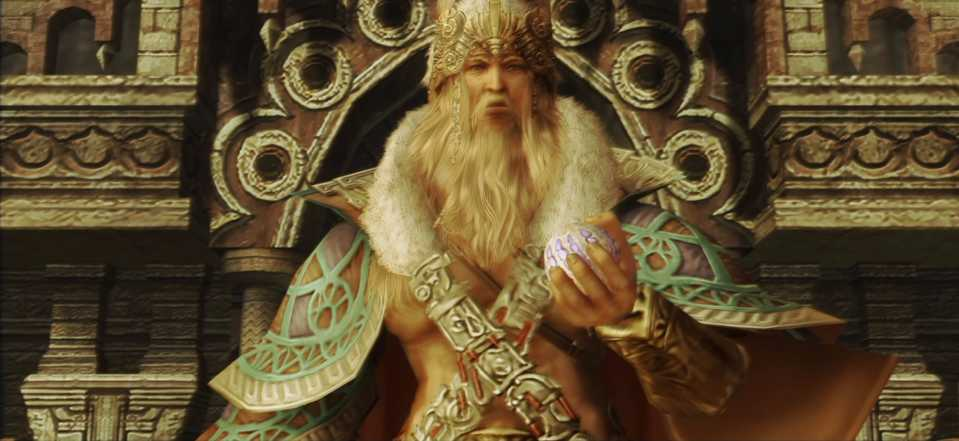
\includegraphics[width=\columnwidth]{./art/tombofraithwall/raithwall.jpg}
%
\vfill
%
After solving the puzzle in this room and making their way back to the Royal Chamber, they notice that another one of the two engravings on the sealed door has now started glowing.
At this point, the previously locked door leading to the Chamber of First Light can now be opened.
As they step through the door, all party members have to perform a DC~8 and everyone who succeeds gets a feeling that they are being watched but they cannot figure out why.
%
\clearpage
%
%
\ofquote{"My family tells a story of the dynast-king and an esper. The story goes that in his youth, the dynast-king defeated a mighty gigas. For which the gods took heed of him. Thereafter, it was bound to him in thralldom."\\}{Ashe}
%
\\\\
%
Stepping out of the Royal Chamber, the party finds themselves in a corridor with three doors.
As they take the door on the left hand side, the party enters an ancient library.
However, none of the many books seem to have withstood the test of time and the party is unable to find any readable ones.
Moreover, the room contains two wooden chest, that can both be opened easily.
Inside the first one, the party finds an X-Potion, a Phoenix Down and a Turbo Ether.
In the other chest, the party finds a heavy book that appears to be in a much better condition than the other ones in the library.
The book seems to tell the story of \accf{Belias the Gigas} and even though most of it is unreadable, with some effort, the party is able to make out the following excerpt:
%
\\\\
%
"Called the Gigas for his appearance: man and monster fused as one. Considered a mistake upon his making, and receiving not his intended role, the Gigas challenged the gods and lost. Scorned by his masters, he found another: the Dynast-King, whose tomb he swore to protect for eternity."
%
\vfill
%
By passing through the door on the right hand side of the corridor, the party enters what seems to be a small armory, with weapon and armor racks scattered across the room.
Unfortunately, most of the equipment found in this room has become unusable, because they have been locked up here for many years, but the party is still able to salvage some particularly durable pieces. 
As such, the party finds the following Advanced level equipment pieces: an Oracle Bone, a Nemean Lionskin and a Trident.
In case the party cannot use some of these equipment pieces, feel free to exchange them for ones that are useful to them.
%
\vfill
%
At the end of the corridor, the party enters a massive hall, the \accf{Chamber of First Light}.
On its opposite end, a wide stairway leads to an altar on which the players see the statue of a four-armed giant with ram-like horns that is sitting with a decorated spear by its side.
Furthermore, the hall is supported by various decorated pillars, similar to the ones found at the entrance of the tomb.
All characters capable of using Magic feel a vast amount of magical energy flowing through the hall.
As the party moves closer to the stairway, the statue of the giant comes to life, slowly stands up and grabs its weapon to attack the party!
%
\newpage
%
\ofmonster{Belias}{5}{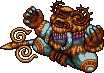
\includegraphics[width=0.32\columnwidth]{./art/tombofraithwall/belias.jpg}}
{
	HP: & \hfill 90 & MP: & \hfill 150\\
	STR: & \hfill 4 & DEF: & \hfill 2 \\
	MAG: & \hfill 5 & RES: & \hfill 3 \\
	AGI: & \hfill 2 & Size: & \hfill L\\
}
{	
	\accf{Spear}: 2d DMG, 2u Range \hfill \accf{Drops:} 1000G\\
	\accf{Resilient}:\earth\fire\dark\holy \hfill \accf{Immune}:\poison\sleep\silence\blind
}
{
	\mspell{Painflare}{20}{1r}{3u}{Self}{All enemies in the target area suffer 4d fire damage.}{\fire}
	\mspell{Firaga}{12}{1r}{Single}{5u}{You deal 6d fire damage to the target.}{\fire}
	\mspell{Greater Barrier}{10}{1r}{Single}{5u}{You gain EnDEF and EnRES for 3 rounds.}{}
	\mpassive{Auto-Haste}{Take two actions on each turn.}
}
%
\vfill
%
After being defeated, Belias disintegrates in a sea of flames.
The party now notices that the absence of the statue reveals another small chamber.
Inside the it stands a golden sarcophagus containing the remains of King Raithwall.
Various chests are spread around the room, containing gold and jewels with a total value of 15000G.
In addition, a decorated pedestal stands in front of the sarcophagus on which lies a glowing orb-like object, the Dawn Shard.
The Dawn Shard is an artifact that can bend the fabric of reality in subtle ways and it can be equipped as an Accessory with the following effect: whenever you perform a check, you may spend any Fortune Die from your pool to re-roll the result instead of exchanging a die.
%
\vfill
%
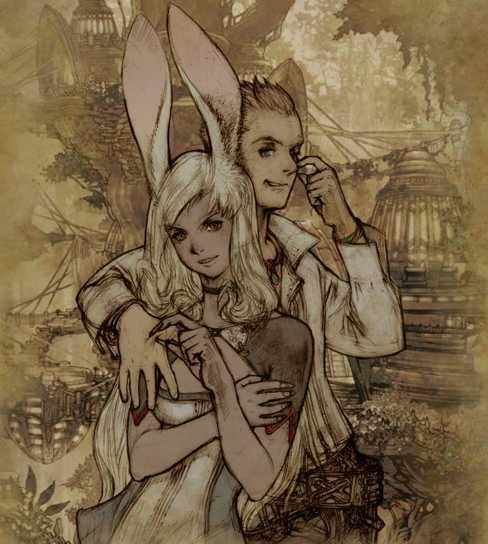
\includegraphics[width=\columnwidth]{./art/tombofraithwall/franandbalthier.jpg}
%
\clearpage
%
As they examine the Dawn Shard, the party suddenly hears the sound of a slow clap behind them and when they turn around, they see two people standing at the entrance of the hall.
They reveal themselves as \accf{Fran and Balthier}.
Balthier is a handsome young man with short brown hair and fancy clothing.
Furthermore, he is very charismatic and cunning, making him almost impossible to trick.
Fran is very tall with an athletic build, long white hair and she is wearing a dark, revealing light armor.
Although she looks mostly humanoid, Fran possesses many distinct feline features such as her long ears and claw-like hands.
Socially, she is almost the polar opposite of her partner as she stays quiet and passive most of the time, observing the situation from a distance.
Fran and Balthier are wanted criminals, while Balthier seems solely motivated by the pursuit of money and wealth, Fran is willing to follow his lead.
Nevertheless, they are not inherently malicious or violent.
Balthier opens the conversation by congratulating the party for making it this far. 
He reveals that the two have entered the tomb after the party and have been following them ever since, making them do all the dirty work.
Balthier then asks the party to hand over the treasure and the Dawn Shard if they want to leave the tomb alive.
At this point, there are different decisions the party can make, some of which are discussed below.
Still, you likely have to improvise some aspects of this final section.
%
\vfill
%
\accf{Don't hand over anything:}
Even though they were hoping to avoid this situation, Fran and Balthier immediately draw their weapons and attack the party, gaining the first turn in the ensuing fight.
During the battle, they focus on keeping their distance and utilizing their ranged weapons.
When necessary, they temporarily hide in other parts of the tomb, hoping to catch members of the party off guard.
In case the entire party suffers KO, Fran and Balthier will not kill them, but leave them unconscious. 
As they awake many hours later, they notice that the two are gone together with the treasure and the Dawn Shard.
In case the party wins the battle, they may decide the fate of Fran and Balthier.
They may for example decide to finish them off, leave them unconscious or they may convince them to join their cause, which the two accept as they have no other choice.
Furthermore, the party can keep both the treasure and the Dawn Shard.
%
\vfill
%
\accf{Hand over the treasure, but keep the Dawn Shard:}
In this case, Fran notes that the Dawn Shard, despite still being a powerful artifact, seems to have lost most of its original power.
Therefore, she suggests that they should agree to the deal to avoid a fight.
Balthier agrees, they pack up the treasure and both parties leave the tomb to go their separate ways.
%
\newpage
%
\accf{Convince them to join forces:}
The party may try to convince Fran and Balthier to join their party.
To succeed in this endeavor, they have to make the the two believe that they can achieve great profit and wealth as members of the party.
Any argument that does not promise a significantly increased bottom line does not convince them at all.
If the party manages to make a reasonable but not fully convincing case for their proposal, they have to make a DC~9 check to determine whether Balthier is persuaded.
They may use the power of their Dawn Shard to improve their odds.
If successful, Fran and Balthier join the party, at least for a while and they are controlled by the GM.
They leave the tomb together with the treasure and the Dawn Shard.
%
\vfill
%
\ofmonster{Balthier}{5}{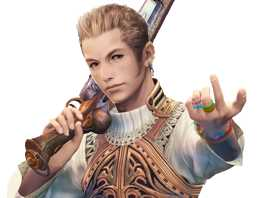
\includegraphics[width=0.3\columnwidth]{./art/tombofraithwall/balthier1.jpg}}
{
	HP: & \hfill 50 & MP: & \hfill 40\\
	STR: & \hfill 4 & DEF: & \hfill 3 \\
	MAG: & \hfill 0 & RES: & \hfill 1 \\
	AGI: & \hfill 2 & Size: & \hfill M\\
}
{\accf{Gun}: 2d DMG, 3u Range}
{
	\mtech{Aim: Legs}{8}{0r}{Single}{Weapon}{Make an Attack against the target and if you hit he additionally suffers Immobile for 1 round.}{}
	\mtech{Big Shot}{6}{0r}{Single}{Weapon}{Make an Attack on the target. If you hit, the damage dealt ignores the target's DEF.}{}
}
%
\vfill
%
\ofmonster{Fran}{5}{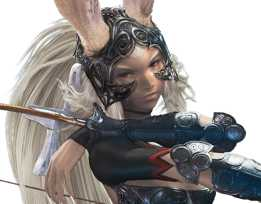
\includegraphics[width=0.28\columnwidth]{./art/tombofraithwall/fran1.jpg}}
{
	HP: & \hfill 45 & MP: & \hfill 45\\
	STR: & \hfill 3 & DEF: & \hfill 3 \\
	MAG: & \hfill 1 & RES: & \hfill 4 \\
	AGI: & \hfill 3 & Size: & \hfill M\\
}
{\accf{Bow}: 2d DMG, 5u Range}
{
	\mtech{Pierceshot}{8}{0r}{10u (line)}{Self}{Make an Attack against all targets in a line, by making one damage roll that applies to all that fail to evade.}{}
	\mtech{Aim: Arm}{8}{0r}{Single}{Weapon}{Make an Attack against the target and if you hit he additionally suffers DeSTR and DeMAG for 1 round.}{}
}
%
\vfill
%
As they step outside, the party feels their eyes burning from the radiant sunlight of the desert, realizing the many hours (or days?) they have spent in the darkness of the tomb.
At the entrance of the Death Valley the party reunites with Dyce, who stares in awe and disbelief upon hearing of the marvels that have played out inside the Tomb of Raithwall.
They stay at his camp for some well deserved rest before moving on to new adventures.
Being the first to march into the Tomb of Raithwall and live to tell the story, the party establishes itself as a force to be reckoned with.
As such, every party member receives a \accf{Level Up}!
%
\clearpage
%
\twocolumn
\colorlet{tombfloor}{yellow!10!white}
\colorlet{tombwall}{white!50!brown}
\colorlet{tombobstacle}{brown}
\colorlet{tombobject}{white!80!black}
%
\begin{figure}[h]
	\centering
	\begin{tikzpicture}[]
	\tikzstyle{stairs}=[fill=tombfloor, ultra thick, draw, trapezium, trapezium angle=85, align=center, pattern=horizontal lines]
	\tikzstyle{pillar}=[ultra thick, draw, circle, align=center, fill=tombobstacle, minimum height=0.05\textwidth]
	\tikzstyle{room}=[fill=tombfloor, ultra thick, draw, rectangle, align=center]
	\tikzstyle{door}=[fill=tombobstacle, ultra thick, draw, rectangle, align=center]
						
	\node[ultra thick, fill=tombwall, draw, rectangle, minimum height=\textheight, minimum width=\textwidth](tarea)at (0,0) {};
			
	\node[fill=yellow!30!white, ultra thick, draw, rectangle, align=center, minimum height=0.2\textheight, minimum width=\textwidth](a1)at (0\textwidth, -0.4\textheight) {};
	
	\node[room, minimum height=0.175\textheight, minimum width=0.7\textwidth](a1)at (0\textwidth, 0.37\textheight) {};
	\node[room, minimum height=0.175\textheight, minimum width=0.8\textwidth](a1)at (0\textwidth, -0.1375\textheight) {};
	\node[room, minimum height=0.05\textheight, minimum width=0.8\textwidth](a1)at (0\textwidth, -0.025\textheight) {};
	\node[room, minimum height=0.28\textheight, minimum width=0.2\textwidth](a1)at (0\textwidth, 0.14\textheight) {};
	
	
	\node[fill=tombfloor, ultra thick, draw, trapezium, trapezium angle=85, align=center, rotate=180, minimum height=0.075\textheight](a1)at (0\textwidth, -0.2625\textheight) {};
	\node[stairs, rotate=180, minimum height=0.075\textheight](a1)at (0\textwidth, -0.2625\textheight) {};
	\node[stairs, minimum height=0.05\textheight](a1)at (-0.3\textwidth, -0.075\textheight) {};
	\node[stairs, minimum height=0.05\textheight](a1)at (0.3\textwidth, -0.075\textheight) {};	
	\node[stairs, pattern=vertical lines, rotate=90, minimum height=0.05\textheight](a1)at (-0.3125\textwidth, 0.37\textheight) {};
	\node[stairs, pattern=vertical lines, rotate=270, minimum height=0.05\textheight](a1)at (0.3125\textwidth, 0.37\textheight) {};
	
	\node[door, minimum height=0.01\textheight, minimum width=0.2\textwidth](a1)at (0\textwidth, 0.28\textheight) {};
	\node[door, minimum height=0.01\textheight, minimum width=0.15\textwidth](a1)at (0\textwidth, 0.455\textheight) {};
	
	\node[pillar, minimum height=0.02\textheight](a1)at (0.2\textwidth, -0.475\textheight) {};
	\node[pillar, minimum height=0.02\textheight](a1)at (0.2\textwidth, -0.4\textheight) {};
	\node[pillar, minimum height=0.02\textheight](a1)at (0.2\textwidth, -0.325\textheight) {};
	\node[pillar, minimum height=0.02\textheight](a1)at (-0.2\textwidth, -0.475\textheight) {};
	\node[pillar, minimum height=0.02\textheight](a1)at (-0.2\textwidth, -0.4\textheight) {};
	\node[pillar, minimum height=0.02\textheight](a1)at (-0.2\textwidth, -0.325\textheight) {};
	
	\node[fill=tombobject, ultra thick, draw, rectangle, align=center, minimum height=0.02\textheight, minimum width=0.2\textwidth](demonwall)at (0\textwidth, -0.05\textheight) {};

	\draw[tombfloor, -, ultra thick](-0.1\textwidth, 0\textheight) -- (0.1\textwidth, 0\textheight);
	\draw[tombfloor, -, ultra thick](0.335\textwidth, -0.05\textheight) -- (0.265\textwidth, -0.05\textheight);
	\draw[tombfloor, -, ultra thick](-0.335\textwidth, -0.05\textheight) -- (-0.265\textwidth, -0.05\textheight);	
	\draw[tombfloor, -, ultra thick](0.355\textwidth, -0.1\textheight) -- (0.245\textwidth, -0.1\textheight);
	\draw[tombfloor, -, ultra thick](-0.355\textwidth, -0.1\textheight) -- (-0.245\textwidth, -0.1\textheight);


	\node[align=center](a2)at (0.4\textwidth, -0.4\textheight) {\bf\LARGE Death \\\\ \bf\LARGE Valley};	
	\node[align=center](a2)at (0.25\textwidth, 0.075\textheight) {\bf\LARGE Hall of the \\\\ \bf\LARGE Destroyer};
		
	\node[align=center](a2)at (0.425\textwidth, 0.37\textheight) {\bf\Large To \\ \bf\Large Northfall \\ \bf\Large Passage};
	\node[align=center](a2)at (-0.425\textwidth, 0.37\textheight) {\bf\Large To\\ \bf\Large Southfall \\ \bf\Large Passage};
	\node[align=center](a2)at (0\textwidth, 0.33\textheight) {\bf\Large Royal Chamber};
	\node[align=center](a2)at (0\textwidth, 0.48\textheight) {\bf\Large To Chamber of First Light};

	\node[align=center](demonwalltext)at (0.1\textwidth, -0.125\textheight) {\bf\Large Demon \\ \bf\Large Wall};
	\draw[->, ultra thick](demonwalltext) -- (demonwall);

	\draw[<->, ultra thick, dashed](-0.12\textwidth, 0\textheight) -- (-0.12\textwidth, 0.28\textheight);
	\node[align=center](a2)at (-0.15\textwidth, 0.14\textheight) {\bf\large 15u};
	\draw[<->, ultra thick, dashed](-0.1\textwidth, 0.15\textheight) -- (0.1\textwidth, 0.15\textheight);
	\node[align=center](a2)at (0\textwidth, 0.14\textheight) {\bf\large 5u};

	\end{tikzpicture}
\end{figure}
%
\clearpage
%
\begin{figure}[h]
	\centering
	\begin{tikzpicture}[]
	\tikzstyle{stairs}=[fill=tombfloor, ultra thick, draw, trapezium, trapezium angle=85, align=center, pattern=horizontal lines]
	\tikzstyle{pillar}=[ultra thick, draw, circle, align=center, fill=tombobstacle, minimum height=0.05\textwidth]
	\tikzstyle{room}=[fill=tombfloor, ultra thick, draw, rectangle, align=center]
	\tikzstyle{door}=[fill=tombobstacle, ultra thick, draw, rectangle, align=center]
	\tikzstyle{sarc}=[fill=tombobject, ultra thick, draw, rectangle, align=center, minimum height=0.05\textheight, minimum width=0.05\textwidth]	
	\tikzstyle{chest}=[fill=tombobject, ultra thick, draw, rectangle, align=center]
	\tikzstyle{statue}=[fill=tombobject, ultra thick, draw, circle, align=center, minimum height=0.03\textheight]	
	\tikzstyle{gargoyle}=[fill=tombobject, ultra thick, draw, circle, align=center, minimum height=0.04\textheight]	
	
	\node[ultra thick, fill=tombwall, draw, rectangle, minimum height=\textheight, minimum width=\textwidth](tarea)at (0,0) {};
	\node[align=center](text)at (0\textwidth, -0.45\textheight) {\bf\LARGE To Royal \bf\LARGE Chamber};
	
	% northfall	
	\node[align=center](text)at (-0.25\textwidth, 0.475\textheight) {\bf\LARGE Northfall Passage};
	\node[fill=tombfloor, ultra thick, draw, trapezium, trapezium angle=85, align=center, minimum height=0.05\textheight](a1)at (-0.3\textwidth, -0.425\textheight) {};	
	\node[stairs, minimum height=0.05\textheight](a1)at (-0.3\textwidth, -0.425\textheight) {};	
	
	\node[room, minimum height=0.3\textheight, minimum width=0.3\textwidth](a1)at (-0.3\textwidth, -0.25\textheight) {};
	\node[room, pattern=checkerboard, pattern color=gray, draw=none, minimum height=0.25\textheight, minimum width=0.298\textwidth](a1)at (-0.299\textwidth, -0.226\textheight) {};
	\node[room, minimum height=0.3\textheight, minimum width=0.3\textwidth](a1)at (-0.3\textwidth, 0.05\textheight) {};
	\node[room, minimum height=0.25\textheight, minimum width=0.4\textwidth](a1)at (-0.25\textwidth, 0.325\textheight) {};	
	\node[room, minimum height=0.5\textheight, minimum width=0.1\textwidth](a1)at (-0.1\textwidth, -0.05\textheight) {};
	\node[room, minimum height=0.1\textheight, minimum width=0.1\textwidth](a1)at (-0.1\textwidth, -0.35\textheight) {};
	
	\node[door, minimum height=0.01\textheight, minimum width=0.1\textwidth](a1)at (-0.35\textwidth, -0.1\textheight) {};
	\node[door, rotate=90, minimum height=0.01\textheight, minimum width=0.1\textwidth](a1)at (-0.15\textwidth, 0.15\textheight) {};
	\node[door, minimum height=0.01\textheight, minimum width=0.1\textwidth](a1)at (-0.35\textwidth, 0.2\textheight) {};
		
	\node[sarc](a1)at (-0.25\textwidth, -0.025\textheight) {};
	\node[sarc](a1)at (-0.37\textwidth, -0.025\textheight) {};
	\node[sarc](a1)at (-0.25\textwidth, 0.05\textheight) {};
	\node[sarc](a1)at (-0.37\textwidth, 0.05\textheight) {};
	\node[sarc](a1)at (-0.25\textwidth, 0.125\textheight) {};
	\node[sarc](a1)at (-0.37\textwidth, 0.125\textheight) {};
		
	\node[chest, minimum height=0.01\textheight, minimum width=0.1\textwidth](a1)at (-0.1\textwidth, -0.3\textheight) {};
	\node[chest, minimum height=0.025\textwidth, minimum width=0.025\textwidth](a1)at (-0.1\textwidth, -0.35\textheight) {};
	\node[chest, fill=brown, minimum height=0.04\textheight, minimum width=0.025\textwidth](a1)at (-0.075\textwidth, -0.05\textheight) {};
	\node[chest, minimum height=0.04\textheight, minimum width=0.025\textwidth](a1)at (-0.075\textwidth, -0.15\textheight) {};
	
	\node[statue](a1)at (-0.25\textwidth, 0.375\textheight) {};
	\node[chest, minimum height=0.025\textheight, minimum width=0.1\textwidth](a1)at (-0.25\textwidth, 0.325\textheight) {};
		
	%southfall
	\node[fill=tombfloor, ultra thick, draw, trapezium, trapezium angle=85, align=center, minimum height=0.05\textheight](a1)at (0.3\textwidth, -0.425\textheight) {};	
	\node[stairs, minimum height=0.05\textheight](a1)at (0.3\textwidth, -0.425\textheight) {};	
	\node[align=center](text)at (0.25\textwidth, 0.475\textheight) {\bf\LARGE Southfall Passage};
	\node[room, minimum height=0.85\textheight, minimum width=0.4\textwidth](a1)at (0.25\textwidth, 0.025\textheight) {};
	\node[room, minimum height=0.05\textheight, minimum width=0.3\textwidth](a1)at (0.3\textwidth, 0.175\textheight) {};
	\node[door, minimum height=0.01\textheight, minimum width=0.1\textwidth](a1)at (0.1\textwidth, 0.155\textheight) {};
	\node[chest, minimum height=0.01\textheight, minimum width=0.1\textwidth](a1)at (0.35\textwidth, 0.155\textheight) {};

	\node[statue](a1)at (0.25\textwidth, 0.375\textheight) {};
	\node[chest, minimum height=0.025\textheight, minimum width=0.1\textwidth](a1)at (0.25\textwidth, 0.325\textheight) {};

	\node[gargoyle](a1)at (0.125\textwidth, -0.25\textheight) {};
	\node[gargoyle](a1)at (0.125\textwidth, -0.1\textheight) {};
	\node[gargoyle](a1)at (0.125\textwidth, 0.05\textheight) {};
	\node[gargoyle](a1)at (0.375\textwidth, -0.25\textheight) {};
	\node[gargoyle](a1)at (0.375\textwidth, -0.1\textheight) {};
	\node[gargoyle](a1)at (0.375\textwidth, 0.05\textheight) {};
	\draw[-, color=red!65!black, ultra thick](0.155\textwidth, -0.25\textheight) -- (0.345\textwidth, -0.25\textheight);
	\draw[-, color=red!65!black, ultra thick](0.155\textwidth, -0.1\textheight) -- (0.345\textwidth, -0.1\textheight);
	\draw[-, color=red!65!black, ultra thick](0.155\textwidth, 0.05\textheight) -- (0.345\textwidth, 0.05\textheight);
	
	\node[chest, minimum height=0.04\textheight, minimum width=0.025\textwidth](a1)at (0.2\textwidth, 0.175\textheight) {};
	
	\end{tikzpicture}
\end{figure}
%
\clearpage
%
\begin{figure}[h]
	\centering
	\begin{tikzpicture}[]
	\tikzstyle{stairs}=[fill=tombfloor, ultra thick, draw, trapezium, trapezium angle=85, align=center, pattern=horizontal lines]
	\tikzstyle{pillar}=[ultra thick, draw, circle, align=center, fill=tombobstacle, minimum height=0.05\textwidth]
	\tikzstyle{room}=[fill=tombfloor, ultra thick, draw, rectangle, align=center]
	\tikzstyle{stairs2}=[fill=yellow!20!white, ultra thick, draw, rectangle, align=center]
	\tikzstyle{door}=[fill=tombobstacle, ultra thick, draw, rectangle, align=center]
	\tikzstyle{sarc}=[fill=tombobject, ultra thick, draw, rectangle, align=center, minimum height=0.05\textheight, minimum width=0.05\textwidth]	
	\tikzstyle{chest}=[fill=tombobject, ultra thick, draw, rectangle, align=center]
	\tikzstyle{statue}=[fill=tombobject, ultra thick, draw, circle, align=center, minimum height=0.03\textheight]	
	\tikzstyle{gargoyle}=[fill=tombobject, ultra thick, draw, circle, align=center, minimum height=0.035\textheight]	
	
	\node[ultra thick, fill=tombwall, draw, rectangle, minimum height=\textheight, minimum width=\textwidth](tarea)at (0,0) {};
	\node[room, minimum height=0.9\textheight, minimum width=0.9\textwidth](a1)at (0\textwidth, 0\textheight) {};	

	%stairs
	\node[stairs2, minimum height=0.225\textheight, minimum width=0.65\textwidth](a1)at (0\textwidth, 0.3375\textheight) {};	
	\node[stairs2, minimum height=0.2\textheight, minimum width=0.60\textwidth](a1)at (0\textwidth, 0.35\textheight) {};	
	\node[stairs2, minimum height=0.175\textheight, minimum width=0.55\textwidth](a1)at (0\textwidth, 0.3625\textheight) {};	
	\node[stairs2, minimum height=0.05\textheight, minimum width=0.5\textwidth](a1)at (0\textwidth, 0.325\textheight) {};	

	\node[room, minimum height=0.3\textheight, minimum width=0.4\textwidth](a1)at (-0.25\textwidth, -0.3\textheight) {};	
	\node[room, minimum height=0.3\textheight, minimum width=0.4\textwidth](a1)at (0.25\textwidth, -0.3\textheight) {};	
	\node[room, minimum height=0.1\textheight, minimum width=0.5\textwidth](a1)at (0\textwidth, 0.4\textheight) {};	
	
	\node[door, minimum height=0.01\textheight, minimum width=0.1\textwidth](a1)at (0\textwidth, 0.35\textheight) {};
	\node[door, minimum height=0.01\textheight, minimum width=0.1\textwidth](a1)at (0\textwidth, -0.445\textheight) {};
	\node[door, minimum height=0.01\textheight, minimum width=0.1\textwidth](a1)at (0\textwidth, -0.155\textheight) {};
	\node[door, rotate=90, minimum height=0.01\textheight, minimum width=0.1\textwidth](a1)at (0.05\textwidth, -0.3\textheight) {};
	\node[door, rotate=90, minimum height=0.01\textheight, minimum width=0.1\textwidth](a1)at (-0.05\textwidth, -0.3\textheight) {};
	
	\node[gargoyle](a1)at (0\textwidth, 0.325\textheight) {};
	\node[align=center](text)at (0\textwidth, -0.475\textheight) {\bf\LARGE To Royal Chamber};
	\node[align=center](text)at (0\textwidth, -0\textheight) {\bf\LARGE Chamber of \\\\ \bf\LARGE First Light};
	
	\node[pillar](a1)at (-0.25\textwidth, -0.1\textheight) {};
	\node[pillar](a1)at (-0.25\textwidth, 0.05\textheight) {};
	\node[pillar](a1)at (-0.25\textwidth, 0.2\textheight) {};
	\node[pillar](a1)at (0.25\textwidth, -0.1\textheight) {};
	\node[pillar](a1)at (0.25\textwidth, 0.05\textheight) {};
	\node[pillar](a1)at (0.25\textwidth, 0.2\textheight) {};
	
	\node[chest, minimum height=0.025\textheight, minimum width=0.15\textwidth](a1)at (0\textwidth, 0.43\textheight) {};
	\node[chest, minimum height=0.02\textheight, minimum width=0.04\textwidth](a1)at (0\textwidth, 0.4\textheight) {};	
	\node[door, minimum height=0.075\textheight, minimum width=0.04\textwidth](a1)at (0.2\textwidth, 0.4\textheight) {};
	\node[door, minimum height=0.075\textheight, minimum width=0.04\textwidth](a1)at (-0.2\textwidth, 0.4\textheight) {};
		
	%library
	\node[chest, minimum height=0.05\textheight, minimum width=0.04\textwidth](a1)at (-0.4\textwidth, -0.4\textheight) {};
	\node[chest, minimum height=0.05\textheight, minimum width=0.04\textwidth](a1)at (-0.4\textwidth, -0.325\textheight) {};
	\node[door, minimum height=0.075\textheight, minimum width=0.04\textwidth](a1)at (-0.4\textwidth, -0.235\textheight) {};
	\node[door, minimum height=0.02\textheight, minimum width=0.3\textwidth](a1)at (-0.225\textwidth, -0.165\textheight) {};
	\node[door, minimum height=0.02\textheight, minimum width=0.2\textwidth](a1)at (-0.2\textwidth, -0.425\textheight) {};
	
	%armory
	\node[chest, minimum height=0.025\textheight, minimum width=0.1\textwidth](a1)at (0.375\textwidth, -0.175\textheight) {};
	\node[door, minimum height=0.04\textheight, minimum width=0.15\textwidth](a1)at (0.2\textwidth, -0.175\textheight) {};
	\node[pillar, minimum height=0.03\textwidth](a1)at (0.2\textwidth, -0.25\textheight) {};	
	\node[pillar, minimum height=0.03\textwidth](a1)at (0.3\textwidth, -0.25\textheight) {};
	\node[pillar, minimum height=0.03\textwidth](a1)at (0.2\textwidth, -0.35\textheight) {};	
	\node[pillar, minimum height=0.03\textwidth](a1)at (0.3\textwidth, -0.35\textheight) {};	
	\node[door, minimum height=0.015\textheight, minimum width=0.3\textwidth](a1)at (0.25\textwidth, -0.435\textheight) {};
		
	\end{tikzpicture}
\end{figure}
%
\clearpage
%
%  And there was i thinking this was going to be hard! - balthier
% He thinks ever and always on his own profit,. Assure him of it, and he shall remain true to our cause. - ashe
% i can hear its call - fran